\chapter{Results}

\section{Results for CNN}
\label{ch:results}
Evaluating the performance of a Convolutional Neural Network (CNN) subjected to varying levels of Gaussian noise, using accuracy as the primary metric. The analysis uses three datasets: training, validation, and testing, to observe how the CNN copes with noise during different phases of model usage.

\begin{figure}[htbp]
  \centering
  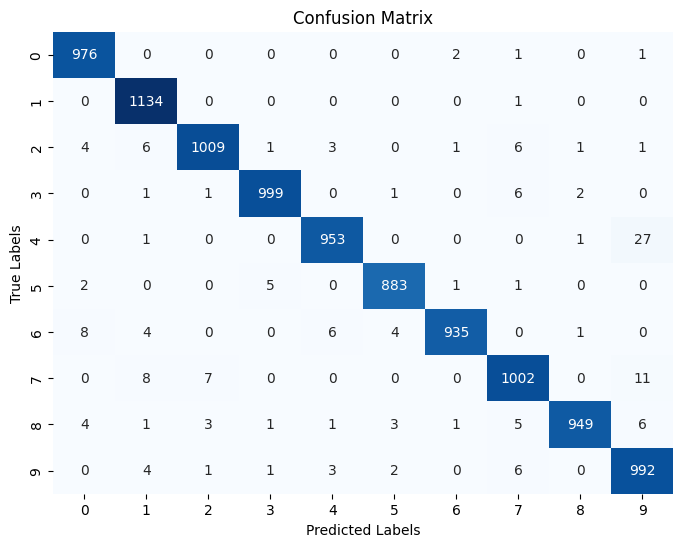
\includegraphics[width=0.7\textwidth]{figures/NL5_Confusionmatrix.png}
  \caption{Confusion Matrix for Noise level 0.5}
  \label{fig:nl5_cm}
\end{figure}


\begin{figure}[htbp]
  \centering
  \begin{minipage}{0.49\textwidth}
    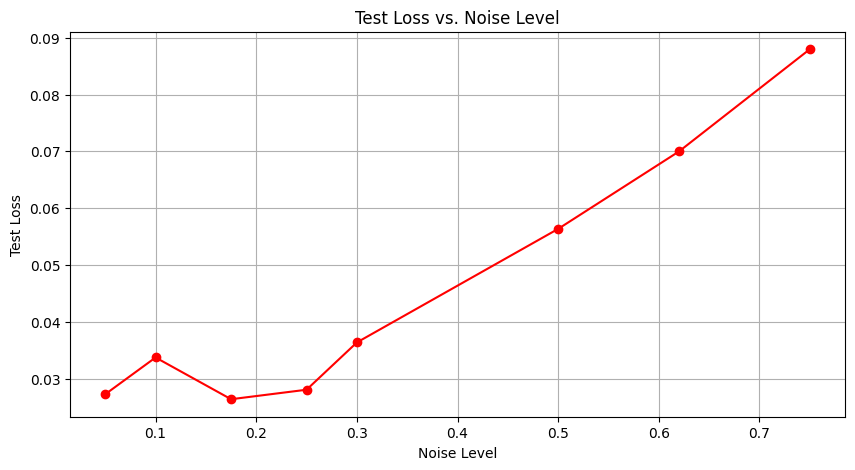
\includegraphics[width=\linewidth]{figures/cnn_testloss.png}
    \caption{CNN Test Loss}
    \label{fig:cnn_testloss}
  \end{minipage}\hfill
  \begin{minipage}{0.49\textwidth}
    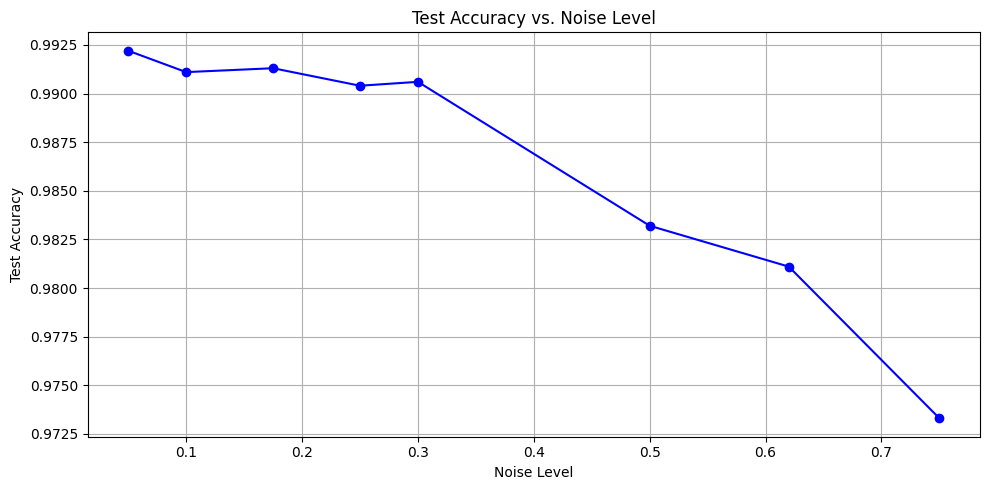
\includegraphics[width=\linewidth]{figures/cnn_testaccuracy.png}
    \caption{CNN Test Accuracy}
    \label{fig:cnn_testaccuracy}
  \end{minipage}
\end{figure}


\begin{table}[h!]
    \centering
    
    \begin{tabular}{|c|c|c|c|c|c|c|c|c|}
        \hline
        \multirow{2}{*}{CNN} & \multicolumn{8}{c|}{Noise Level} \\ \cline{2-9}
                             & 0.05 & 0.1 & 0.175 & 0.25 & 0.3 & 0.5 & 0.62 & 0.75 \\ \hline
        Training              & 99.56\% & 99.55\%  & 99.65\%  & 99.42\%  & 99.18\%  & 98.35\%  & 97.17\%  & 93.88\%  \\ \hline
        Validation            & 98.65\% & 98.77\% & 99.02\%  & 98.07\% & 98.08\% & 96.28\% & 94.46\% & 89.99\% \\ \hline
        Testing               & 98.99\% & 99.07\% & 98.98\%  & 98.91\% & 98.84\% & 98.54\% & 98.46\% & 97.74\% \\ \hline
    \end{tabular}
    \caption{CNN Accuracy Across Different Noise Levels}
\end{table}

The testing accuracy starts at a high of 98.99\% with minimal noise and remains robust up to a noise level of 0.5.



\section{Results for DAE}
The performance of a Denoising Autoencoder (DAE) when exposed to varying levels of Gaussian noise, evaluating its efficiency using reconstruction mean squared error (MSE) for assessing the quality of image reconstruction and training and validation losses to gauge model learning performance.

\begin{figure}[htbp]
  \centering
  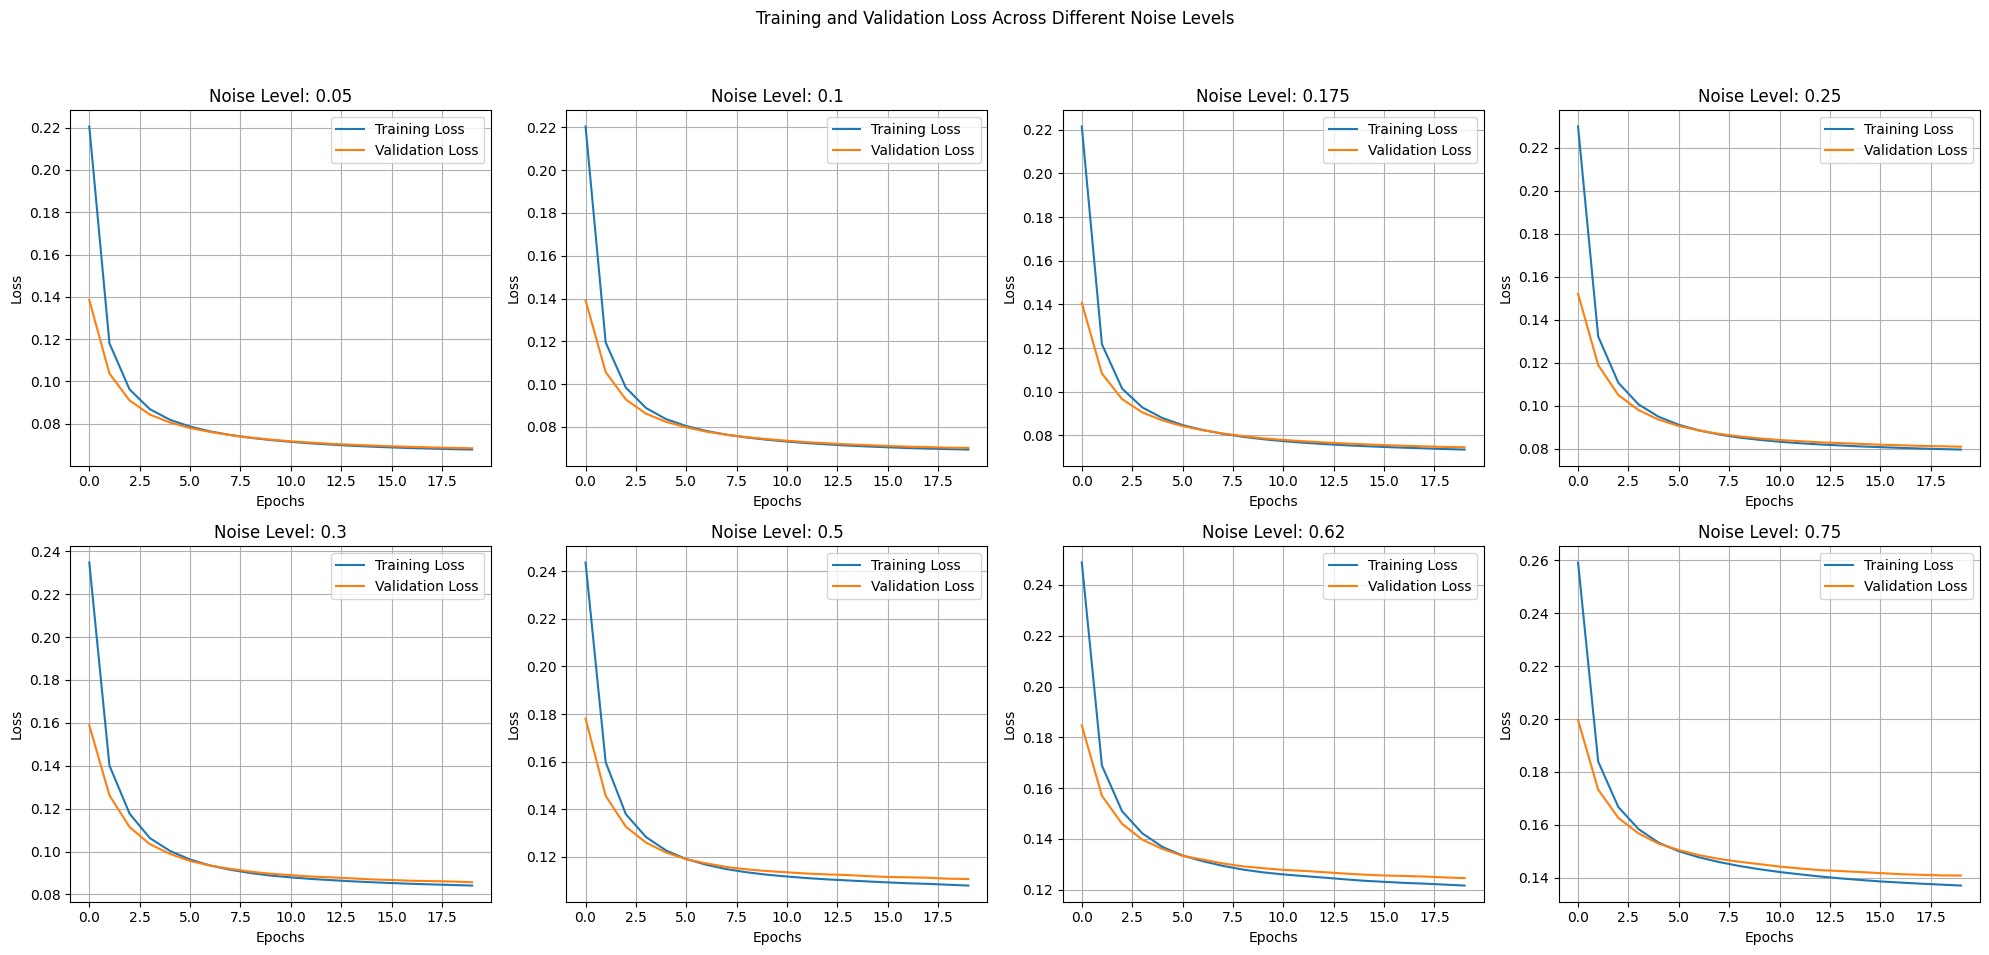
\includegraphics[width=0.8\textwidth]{figures/dae_TVloss.png}
  \caption{Training \& Validation Loss on various noise levels}
  \label{fig:dae_tvloss}
\end{figure}


\begin{figure}[htbp]
  \centering
  \begin{minipage}{0.49\textwidth}
    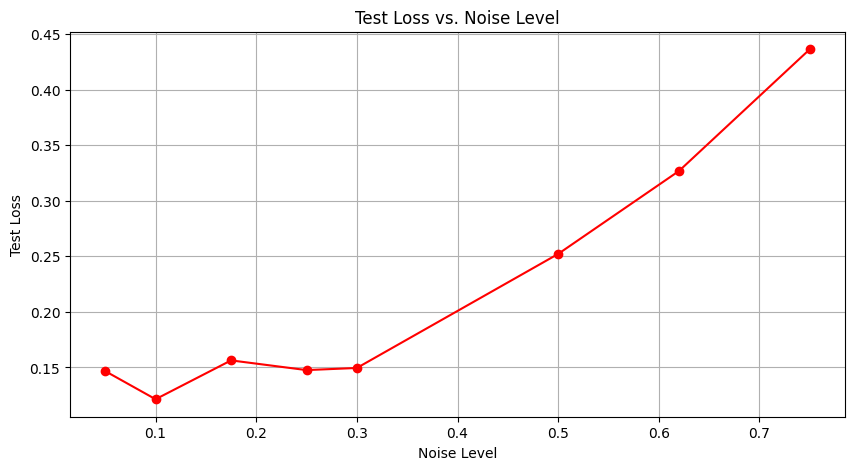
\includegraphics[width=\linewidth]{figures/dae_testloss.png}
    \caption{DAE Classifier Test Loss}
    \label{fig:dae_testloss}
  \end{minipage}\hfill
  \begin{minipage}{0.49\textwidth}
    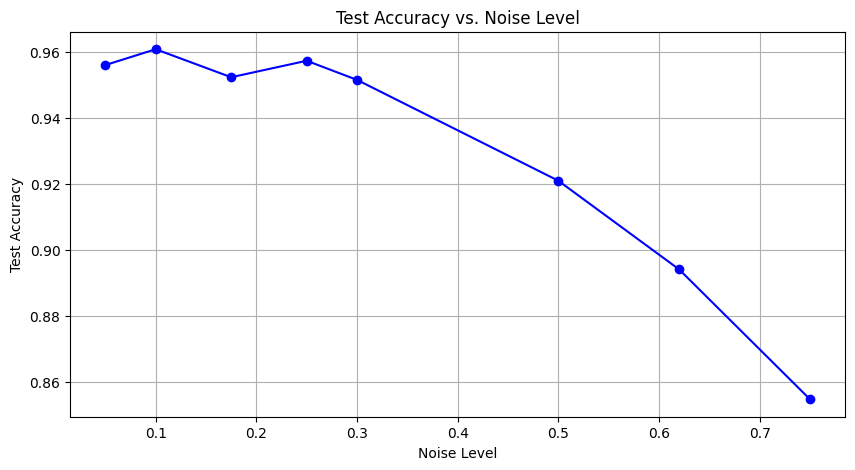
\includegraphics[width=\linewidth]{figures/dae_testaccuracy.png}
    \caption{DAE Classifier Test Accuracy}
    \label{fig:dae_testaccuracy}
  \end{minipage}
\end{figure}

\vspace*{1.2in}

\begin{table}[ht]
\centering
\label{tab:dae_performance}
\begin{tabular}{c|c|c|c}
\toprule
\textbf{Noise Level} & \textbf{Reconstruction MSE} & \textbf{Training Loss} & \textbf{Validation Loss} \\
\midrule
0.05 & 0.0021 & 0.0678 & 0.0684 \\
0.10 & 0.0026 & 0.0695 & 0.0702 \\
0.175 & 0.0038 & 0.0735 & 0.0746 \\
0.25 & 0.0057 & 0.0796 & 0.0809 \\
0.30 & 0.0072 & 0.0841 & 0.0857 \\
0.50 & 0.0148 & 0.1079 & 0.1106 \\
0.62 & 0.0195 & 0.1216 & 0.1245 \\
0.75 & 0.0249 & 0.1386 & 0.1418 \\
\bottomrule
\end{tabular}
\caption{Performance of Denoising Autoencoder (DAE) at Different Noise Levels}
\end{table}

\begin{figure}[htbp]
  \centering
  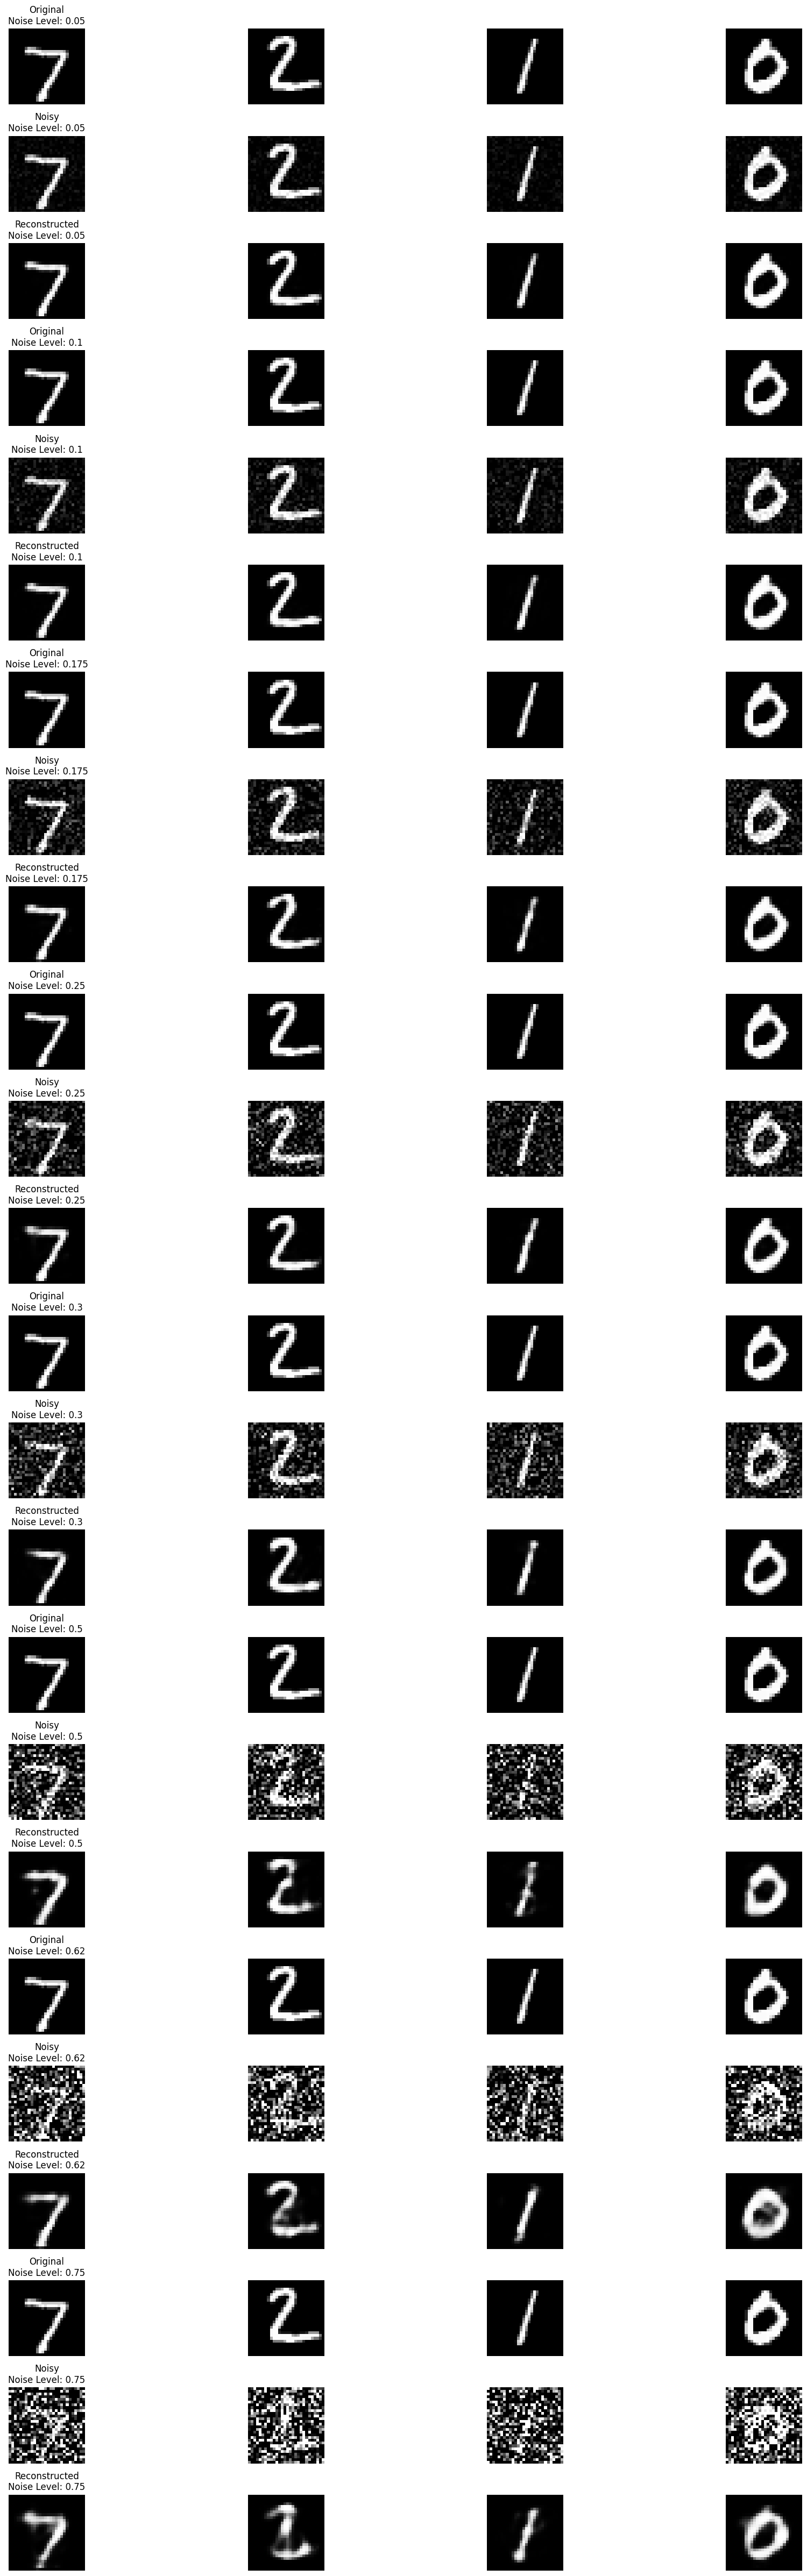
\includegraphics[width=0.8\textwidth]{figures/reconstructed_images.png}
  \caption{DAE Image Reconstruction on various noise levels}
  \label{fig:dae_imgreconst}
\end{figure}

\subsubsection{Image Reconstruction using DAE}
The image showcases a Denoising Autoencoder's (DAE) performance in cleaning digit images across a spectrum of Gaussian noise intensities. The format is arranged in a descending order of noise levels, with original images at the top, followed by noisy versions, and concluding with the DAE's reconstructed outputs at the bottom of each set. At lower noise levels, the DAE effectively restores the digits to a state closely resembling the originals. However, as noise intensifies, the quality of reconstruction degrades, revealing the DAE's decreasing ability to accurately denoise the images, especially when the noise reaches the highest levels. This visual demonstration effectively highlights the DAE's strengths in mitigating noise and its challenges in handling extreme noise conditions.



As shown in \ref{tab:dae_classifier_accuracy}  table presents the classification test accuracy of a Denoising Autoencoder (DAE) classifier at various noise levels, illustrating how the DAE's performance is affected as the noise level increases. Initially, at low noise levels (0.05 to 0.30), the DAE maintains high accuracy, slightly fluctuating but staying above 95\%. This indicates the DAE's strong capability to accurately classify images with minimal to moderate noise. However, as the noise level rises to 0.50 and beyond, there is a clear downward trend in accuracy, with a notable drop to 85.47\% at a noise level of 0.75. These figures underscore the challenge that higher noise levels pose to the DAE's classification ability, highlighting a decrease in performance as the noise approaches higher intensities.

\begin{table}[ht]
\centering
\begin{tabular}{c|c}
\toprule
\textbf{Noise Level} & \textbf{Accuracy (\%)} \\
\midrule
0.05 & 95.60\% \\
0.10 & 96.09\% \\
0.175 & 95.24\% \\
0.25 & 95.74\% \\
0.30 & 95.16\% \\
0.50 & 92.10\% \\
0.62 & 89.41\% \\
0.75 & 85.47\% \\
\bottomrule
\end{tabular}
\caption{Classification Test Accuracy of DAE Classifier at Various Noise Levels}
\label{tab:dae_classifier_accuracy}
\end{table}

\section{Summary}
The robustness and adaptability of both the Convolutional Neural Network (CNN) and the Denoising Autoencoder (DAE) when challenged by varying levels of Gaussian noise. The CNN maintains high accuracy across training, validation, and testing phases with minimal degradation until noise levels reach 0.5, demonstrating effective noise resilience. Conversely, the DAE, assessed through reconstruction MSE and training/validation losses, shows a gradual increase in error as noise levels rise, indicating a decline in its ability to reconstruct images precisely at higher noise intensities. Additionally, the classification accuracy of a DAE-based classifier also declines as noise increases, further illustrating the challenges faced by DAEs in maintaining performance under severe noise conditions. Together, these results highlight the strengths and limitations of both models in noise-affected environments, guiding potential improvements for noise robustness in neural network applications.



